All questions related to orthogonality, norm, distance, etc. in the following exercises are always understood to be with regard to the given inner product. 
\bb
\ii Let $(V, \angvec{ , })$ be an inner product space, and let $W\subseteq V$ be a subspace. Show that $W^\perp$ is a subspace. 
\\
\begin{solution}
\noindent  \\
(i) Since $\angvec{\boldv,\boldzero}=0$ for {\em any $\boldv$ whatsoever}, we have $\boldzero\in W^\perp$. \\
(ii)+(iii) Suppose $\boldv_1,\boldv_2\in W^\perp$. We must show $c_1\boldv_1+c_2\boldv_2\in W^\perp$ for any $c_1,c_2\in\R$. Given any $\boldw\in W$, we compute 
\begin{align*}
\angvec{\boldw, c_1\boldv_1+c_2\boldv_2}&=c_1\angvec{\boldw,\boldv_1}+c_2\angvec{\boldw,\boldv_2} &\text{(bilinearity}\\
&=c_1\cdot 0+c_2\cdot 0 &\text{(since $\boldv_i\in W^\perp$)}\\
&=0.
\end{align*}  
This proves $c_1\boldv_1+c_2\boldv_2\in W^\perp$, as desired. 
\end{solution}
\ii Let $(V, \angvec{ , })$ be an inner product space, and let $W\subseteq V$ be a subspace. Show that \\ $W\cap W^\perp=\{\boldzero\}$. 
\\
\begin{solution}
\noindent
First observe that $\boldzero_V\in W$ and $\boldzero_V\in W^\perp$, since both are subspaces. It follows that $\boldzero_V\in W\cap W^\perp$ (by def. of $\cap$), and thus that $\{\boldzero_V\}\subseteq W\cap W^\perp$. 
\\
To show the other subset relation, suppose $\boldv\in W\cap W^\perp$. Recall that by definition of $\cap$ this means $\boldv\in W$ and $\boldv\in W^\perp$. Since an element of $W^\perp$ is orthogonal to everything in $W$ we must have $\boldv$ orthogonal to itself. This means $\langle\boldv,\boldv\rangle=0$. By the positivity axiom it now follows that $\boldv=\boldzero_V$. Thus the only element of $W\cap W^\perp$ is $\boldzero_V$, and hence $W\cap W^\perp=\{\boldzero_V\}$. 
\end{solution}

\ii Consider the vector space $V=C([0,1])$ with standard {\em integral inner product}. 
\\
Apply Gram-Schmidt to the basis $B=\{1,2^x, 3^x\}$ of $W=\Span(B)$ to obtain an orthogonal basis of $W$. 
\\
\begin{solution}
\noindent The resulting orthogonal basis is $B'=\{f_1, f_2,f_3\}$, where 
\begin{align*}
f_1&=1 \\
f_2&=2^x-(\angvec{2^x,1}/\angvec{1,1})1\\
     &=2^x-(\int_{0}^12^x \ dx)/(\int_0^1 1 \ dx)=2^x-\frac{1}{\ln 2}\\
f_3&=3^x-(\angvec{3^x,2^x-\frac{1}{\ln 2}}/\angvec{2^x-\frac{1}{\ln 2}, 2^x-\frac{1}{\ln 2}})(2^x-\frac{1}{\ln 2})-(\angvec{3^x,1}/\angvec{1,1})1\\
&=3^x-\frac{\frac{2}{\ln 2\ln 3}+\frac{5}{\ln 6}}{\frac{1}{(\ln 2)^2}+\frac{3}{\ln 4}}(2^x-\frac{1}{\ln 2})-\frac{1}{\ln 3}
\end{align*}
OK, I admit, I used technology to compute those integrals. 
\end{solution}
\ii Consider the vector space $V=P_2$ with the {\em evaluation inner product} 
\[
\angvec{p(x),q(x)}=p(-1)q(-1)+p(0)q(0)+p(1)q(1).
\] 
Apply Gram-Schmidt to the standard basis of $P_2$ to obtain an orthogonal basis of $P_2$. 
\\
\begin{solution}
\noindent Applying Gram-Schmidt to the basis $B=\{1,x,x^2\}$ yields the orthogonal basis 
\[
B'=\left\{p_1=1, p_2=x, p_3=x^2-\frac{2}{3}\right\}.
\]
Here are the steps: 
\begin{align*}
p_1&=1 \\
p_2&=x-\frac{\angvec{x,1}}{\angvec{1,1}}1\\
&=x &\text{(since $\angvec{x,1}=-1+0+1=0$)}\\
p_3&=x^2-\frac{\angvec{x^2,p_2}}{\angvec{p_2,p_2}}p_2-\frac{\angvec{x^2,1}}{\angvec{1,1}}\\
&=x^2-\frac{0}{2}x-\frac{2}{3}1&\left(\begin{array}{c} \angvec{x^2,x}=-1+0+1=0\\ \angvec{x^2,1}=1+0+1=2\\ \angvec{1,1}=1+1+1=3\end{array}\right)\\
&=x^2-\frac{2}{3}
\end{align*}
\end{solution}
\ii Let $V=M_{22}$ with inner product $\angvec{A,B}=\tr(A^TB)$, and let $W\subseteq V$ be the subspace of matrices whose trace is 0. 
\bb
\ii Compute an orthogonal basis for $W$. 
\ii Compute $\proj{A}{W}$, where $A$ is the matrix $A=\begin{bmatrix}
1&2\\
1&1\\
\end{bmatrix}
$
\ee
\begin{solution}
\noindent  
(a) The general element of $W$ looks like $A=\begin{bmatrix}
a&b\\
c&-a
\end{bmatrix}$. From this description we see easily that 
\[
B=\left\{ 
A_1=\begin{bmatrix}
1&0\\
0&-1
\end{bmatrix}, 
A_2=\begin{bmatrix}
0&1\\
0&0
\end{bmatrix},
A_3=\begin{bmatrix}
0&0\\
1&0
\end{bmatrix}
\right\}
\]
is a basis for $W$. Furthermore, a simple computation shows this basis is already orthogonal. What luck! 
\\
(b) With the orthogonal basis $B$ in hand, we use the orthogonal projection formula to compute 
\begin{align*}
\proj{A}{W}&=\angvec{A,A_1}/\angvec{A_1,A_1} A_1+\angvec{A,A_2}/\angvec{A_2,A_2} A_2+\angvec{A,A_3}/\angvec{A_3,A_3} A_3\\
&=0A_1+2A_2+A_3\\
&=\begin{bmatrix}
0&2\\
1&0
\end{bmatrix}
\end{align*}
\end{solution}
\ii Let $V=M_{nn}$ with inner product $\angvec{A,B}=\tr(A^TB)$.
\\
Let $W_1$ be the subspace of all symmetric matrices ($A^T=A$), and let $W_2$ be the subspace of all skew-symmetric matrices ($A^T=-A$). 
\\
Recall (from a previous exercise) that $\dim W_1=\frac{n(n+1)}{2}$ and $\dim W_2=\frac{n(n-1)}{2}$. 
\bb
\ii Show that $W_2\subseteq (W_1)^\perp$: i.e., skew-symmetric matrices are orthogonal to symmetric matrices!
\ii Use the result of Exercise \ref{ex:orthcomp} and a dimension argument to show that in fact $W_2=W_1^\perp$. 
\ii Use parts (a)-(b) and the orthogonal projection theorem to show that any matrix $A\in M_{nn}$ can be written uniquely in the form $A=A_1+A_2$, where $A_1$ is a symmetric matrix and $A_2$ is a skew-symmetric matrix. 
\ee
\begin{solution}
\noindent First I reveal a dirty little secret. This ``exotic"  inner product is really nothing more than the dot product in disguise, once we take these rectangular arrays and stretch them out into column vectors! More rigorously, given $A=(a_{ij})$ and $B=(b_{ij})$, we have 
\begin{align*}
\angvec{A,B}&=\tr(A^TB)\\
&=\sum_{k=1}^n \left(A^TB\right)_{kk}\\
&=\sum_{k=1}^n \sum_{\ell=1}^n (A^T)_{k\ell}(B)_{\ell k}\\
&=\sum_{k=1}^n \sum_{\ell=1}^n (A)_{\ell k}(B)_{\ell k}\\
&=\sum_{k=1}^n \sum_{\ell=1}^n a_{\ell k}b_{\ell k}\\
&=\sum_{\substack{1\leq i\leq n\\ 1\leq j\leq n}} a_{ij}b_{ij}
\end{align*}
In other words, the inner product of two matrices is just the sum of the products of their corresponding entries: aka, the dot product! 

Let's use this last formula to compute $\angvec{A,B}$ when $A^T=-A$ and $B^T=B$. First, since skew-symmetric matrices must have 0's along the diagonal, we have $a_{ii}=0$ for all $i$. For $i\ne j$, we have $a_{ji}=-a_{ij}$ and $b_{ji}=b_{ij}$. Then 
\begin{align*}
\angvec{A, B}&=\sum_{\substack{1\leq i\leq n\\ 1\leq j\leq n}} a_{ij}b_{ij}\\
&=\sum_{1\leq i \leq n}a_{ii}b_{ii}+\sum_{1\leq i<j\leq n} a_{ij}b_{ij}+\sum_{1\leq i<j \leq n}a_{ji}b_{ji} &\text{(grouping the terms of the sum any way we like)}\\
&=0+\sum_{1\leq i<j\leq n} a_{ij}b_{ij}+\sum_{1\leq i<j \leq n}-a_{ij}b_{ij} &\text{($a_{ii}=0$, $a_{ji}=-a_{ij}$, $b_{ij}=b_{ji}$)}\\
&=\sum_{1\leq i<j\leq n} a_{ij}b_{ij}-\sum_{1\leq i<j\leq n} a_{ij}b_{ij}\\
&=0.
\end{align*}
Here's an alternative, slightly slicker approach. First observe that in general $\tr(AB)=\tr(BA)$. This is a somewhat surprising property, but follows easily from an argument similar to above: namely, 
\[
\tr(AB)=\sum_{1\leq i, j\leq n} a_{ji}b_{ij}=\sum_{1\leq i\leq j\leq n}b_{ij}a_{ji}=\tr(BA).
\]
Now assume $A^T=-A$ and $B^T=B$. Then 
\begin{align*}
\tr(A^TB)&=\tr\left( (A^TB)^T)\right) &\text{(since transpose doesn't change diagonal)}\\
&=\tr(B^TA) &\text{(prop. of transpose)}\\
&=\tr(AB^T) &\text{(prop. of trace mentioned above)}\\
&=\tr(-A^TB) &\text{(since $A^T=-A$, $B^T=B$)}\\
&=-\tr(A^TB) &\text{(prop. of trace)}
\end{align*}
We've shown $\tr(A^TB)=-\tr(A^TB)$; it follows that $\tr(A^TB)=0$. 
\\
(b) We have $W_2\subseteq W_1^\perp$. By Exercise \ref{ex:orthcomp}, we know $\dim W_1^\perp=\dim M_{nn}-\dim W_1=n^2-\frac{n(n+1)}{2}=\frac{n(n-1)}{2}$. But we've seen in a previous exercise that $\dim W_2=\frac{n(n-1)}{2}$. It follows from the dimension theorem compendium (subspace part) that $W_2=W_1^\perp$. 
\\
(c) By the orthogonal projection theorem, any $A\in M_{nn}$ can be expressed as $A=B+B^\perp$ where $B\in W_1$ and $B^\perp\in W_1^\perp$. We have $W_1$ the space of symmetric matrices, and we just showed that $W_1^\perp$ is the space of skew-symmetric matrices. Thus $B$ is symmetric and $B^\perp$ is skew-symmetric, as desired. 
\end{solution}
\ii Let $V=M_{22}$ with inner product $\angvec{A,B}=\tr(A^TB)$, let $W_1$ be the subspace of symmetric matrices, and let $W_2$ be the subspace of skew-symmetric matrices. 
\begin{samepage}
\bb
\ii Verify that $B_1=\left\{
A_1=\begin{bmatrix}
1&0\\ 0&0
\end{bmatrix},
\begin{bmatrix}
0&1\\
1&0
\end{bmatrix},
A_2=\begin{bmatrix}
0&0\\
0&1
\end{bmatrix}
\right\}$
is an orthogonal basis of $W_1$. 
\\
Verify that $B_2=\left\{ 
A_3=\begin{bmatrix}
0&1\\
-1&0
\end{bmatrix}
\right\}$
is an orthogonal basis of $W_2$. 
\ii Let $A=\begin{bmatrix}
1&2\\
1&1
\end{bmatrix}$. 
\bb
\ii Use the previous exercise and the orthogonal projection formula to write $A=A_1+A_2$, where $A_1$ is symmetric and $A_2$ is skew-symmetric. 
\ii Compute $d(A,W_1)$, the distance from $A$ to the subspace $W_1$. 
\ee
\ee
\end{samepage}
\begin{solution}
\noindent
(a) It is easy to see that the given bases are orthogonal. 
\\
(b) From the previous exercise, we know that the orthogonal decomposition of $A=B+B^\perp$ yields the desired decomposition of $A$ into a sum of a symmetric matrix and skew-symmetric matrix. We use the projection formulas to compute the projections $B$ and $B^\perp$:
\begin{align*}
B&=\proj{A}{W_1}\\
&=\angvec{A,A_1}/\angvec{A_1,A_1} A_1+\angvec{A,A_2}/\angvec{A_2,A_2} A_2+\angvec{A,A_3}/\angvec{A_3,A_3} A_3\\
&=\frac{1}{1}A_1+\frac{3}{2}A_2+\frac{1}{1}A_3\\
&=\begin{bmatrix}
1&\frac{3}{2}\\
\frac{3}{2}&1
\end{bmatrix}
\\
\\
B^\perp&=A-\proj{A}{W_1}\\
&=\begin{bmatrix}
0&\frac{1}{2}\\
-\frac{1}{2}&0
\end{bmatrix}
\end{align*}
Observe that $B$ and $B^\perp$ are indeed symmetric and skew-symmetric, resp., and that $A=B+B^\perp$. 

By definition $d(A, W_1)=\norm{A-B}=\norm{B^\perp}=\sqrt{1/2}=\frac{\sqrt{2}}{2}$.
\end{solution}
\ii Let $V=C([0,1])$ with the standard {\em integral inner product}, and let $f(x)=x$. Find the function of the form $g(x)=a+b\cos(2\pi x)+c\sin(2\pi x)$ that best approximates $f(x)$ (with respect to this inner product). 
\\
\begin{solution}
%\ \\
\noindent 
The given inner product is $\ds \angvec{f,g}=\int_0^1f(x)g(x) \ dx$. The desired function $g$ is simply $\proj{f}{W}$, where $W=\Span\{f_1=1, f_2=\cos(2\pi x), f_3=\sin(2\pi x)\}$. The given functions form an orthogonal basis for $W$ with respect to the given inner product, allowing us to use the orthogonal projection formula:
\begin{align*}
g&=\proj{f}{W}\\
&=\frac{\angvec{f,f_1}}{\angvec{f_1,f_1}}f_1+\frac{\angvec{f,f_2}}{\angvec{f_2,f_2}}f_2+\frac{\angvec{f,f_3}}{\angvec{f_3,f_3}}f_3\\
&=\frac{1}{2}+\frac{0}{1/2}\cos(2\pi x)+\frac{1/2\pi}{1/2}\sin(2\pi x) &\text{(I've omitted all the integral details)}\\
&=\frac{1}{2}+\frac{1}{\pi}\sin(2\pi x).
\end{align*}
\end{solution}
\ii Compute an orthogonal basis of $W$, where $W$ is the plane $x+2y-z=0$. Then extend this orthgonal basis to an orthogonal basis of $\R^3$.
\\
\begin{solution}
\noindent
The plane $W$ is the null space of the matrix $[1 \ 2 \ -1]$. The usual nulls space algorithm produces the basis $\{ (1,0,1), (-2,1,0)\}$ for $W$. Use Gram-Schmidt to convert this to an orthogonal basis $B'=\{ (1,0,1), (-1,1,1)\}$. 

\noindent
To extend $B'$ to a basis of $\R^3$, we need only add another nonzero vector that is orthogonal to both $(1,0,1), (-1,1,1)$. That's easy! Since both vectors are elements of $W$, they are both orthogonal to its defining normal vector $\boldn=(1,2,-1)$. Thus $B''=\{(1,0,1),(-1,1,1),(1,2,-1)\}$ is an orthogonal basis of $\R^3$. 
\end{solution}
\ii Let $A$ be an $n\times n$ matrix. 

Prove: $A^T=A^{-1}$ if and only if the columns of $A$ are an orthonormal basis of $\R^n$. 

Matrices satisfying $A^T=A^{-1}$ are called {\bf orthogonal matrices}. 
\\
\begin{solution}
\ 
\end{solution}
\ii\label{ex:orthproj} Let $V$ an inner product space, and let $W\subseteq V$ be a finite-dimensional subspace. 
\\
Recall that $\proj{\boldv}{W}$ is defined as the unique $\boldw\in W$ satisfying $\boldv=\boldw+\boldw^\perp$, where $\boldw^\perp\in W^\perp$. 
\\
Use this definition (including the uniqueness claim) to prove the following properties: 
\bb
\ii $\proj{c_1\boldv_1+c_2\boldv_2}{W}=c_1\proj{\boldv_1}{W}+c_2\proj{\boldv_2}{W}$ for all $\boldv_1,\boldv_2\in V$ and all $c_1,c_2\in \R$; 
\ii $\boldv\in W\Longleftrightarrow \proj{\boldv}{W}=\boldv$;
\ii $\boldv\in W^\perp\Longleftrightarrow \proj{\boldv}{W}=\boldzero$.

\ee
\begin{solution}
\noindent
(a) By the orthogonal projection theorem we can write 
\begin{align*}
\boldv_1&=\boldw_1+\boldw_1^\perp \hspace{5pt} \text{ where } \boldw_1\in W, \boldw_1^\perp\in W^\perp\\
\boldv_2&=\boldw_2+\boldw_2^\perp \hspace{5pt} \text{ where } \boldw_2\in W, \boldw_2^\perp\in W^\perp.
\end{align*}
By definition, this means $\proj{\boldv_i}{W}=\boldw_i$ for $i=1,2$. Then we have 
\begin{align*}
c_1\boldv_1+c_2\boldv_2&=c_1(\boldw_1+\boldw_1^\perp)+ c_2(\boldw_2+\boldw_2^\perp) \\
&=(c_1\boldw_1+c_2\boldw_2)+(c_1\boldw_1^\perp+c_2\boldw^\perp)
\end{align*}
Since $c_1\boldw_1+c_2\boldw_2\in W$ and $c_1\boldw_1^\perp+c_2\boldw^\perp\in W^\perp$, we recognize 
\[
c_1\boldv_1+c_2\boldv_2=(c_1\boldw_1+c_2\boldw_2)+(c_1\boldw_1^\perp+c_2\boldw^\perp)
\]
as an orthogonal decomposition. It follows, again by definition, that 
\[
\proj{\boldv}{W}=c_1\boldw_1+c_2\boldw_2=c_1\proj{\boldv_1}{W}+c_2\proj{\boldv_2}{W}.
\]
\noindent 
(b) We have 
$\boldv\in W$ if and only if  $\boldv=\boldv+\boldzero$ ($\boldv\in W, \boldzero\in W^\perp$) is the orthogonal decomposition of $\boldv$ with respect to $W$ if and only if $\proj{\boldv}{W}=\boldv$. 
\\
(c) We have 
$\boldv\in W^\perp$ if and only if  $\boldv=\boldzero+\boldv$ ($\boldzero\in W, \boldv\in W^\perp$) is the orthogonal decomposition of $\boldv$ with respect to $W$ if and only if $\proj{\boldv}{W}=\boldzero$. 
\end{solution}
\ii \label{ex:orthcomp}  Let $(V, \ \angvec{\ , \ })$ be an inner product space of dimension $n$, and suppose  $W\subseteq V$ is a subspace of dimension $r$. Prove: $\dim W^\perp=n-r$. 

\noindent
{\bf Hint}: begin by picking an {\em orthogonal} basis $B=\{\boldv_1,\dots ,\boldv_r\}$ of $W$ and extend to an {\em orthogonal} basis $B'=\{\boldv_1,\boldv_2, \dots, \boldv_r, \boldu_1,\dots , \boldu_{n-r}\}$ of all of $V$. Show the $\boldu_i$ form a basis for $W^\perp$.  
\\
\begin{solution}
\noindent Observe first that if we can show all the steps in the hint, then $W^\perp$ has as a basis $B''=\{\boldu_1,\dots, \boldu_{n-r}\}$, and hence $\dim(W^\perp)=n-r$, as desired. 
\\
To show $B''$ is a basis of $W^\perp$ we must show that (1) it is independent, and (2) it spans $W^\perp$. 
\\
Independence is easy: this follows from the fact that the big set $B'$ is independent (in fact orthogonal); any subset of a linearly independent set is itself linearly independent.
\\
Now we show that $B''$ spans $W^\perp$. First note that each $\boldu_i$ is indeed an element of $W^\perp$ since by assumption the set $B'$ is orthogonal. This means that $\langle\boldu_i,\boldv_j\rangle=0$ for all $j$; since the $\boldv_j$ are a basis for $W$, it follows that $\langle\boldu_i,\boldw\rangle=0$ for all $\boldw\in W$. 
\\
Next take any element $\boldu\in W^\perp$. Since $B'$ is a basis of the whole space $V$, we can write $\boldu$ as a linear combination of the $\boldv_i$ and $\boldu_i$:
\[
\boldu=c_1\boldv_1+\cdots +c_r\boldv_r+d_1\boldu_1+\cdots d_{n-r}\boldu_{n-r}.
\]
We will show that each $c_i=0$, and hence that in fact we have 
\[
\boldu=d_1\boldu_1+\cdots d_{n-r}\boldu_{n-r}\in\Span(\{\boldu_1,\dots, \boldu_{n-r}\}). 
\]
To show $c_i=0$ we simply take the inner product of $\boldu$ with $\boldv_i$:
\begin{align*}
0&=\langle\boldu,\boldv_i\rangle &\text{(since $\boldu\in W^\perp$)}\\
&=\langle c_1\boldv_1+\cdots +c_r\boldv_r+d_1\boldu_1+\cdots d_{n-r}\boldu_{n-r},\boldv_i\rangle\\
&=c_1\cancelto{0}{\langle\boldv_1,\boldv_i\rangle}+\cdots c_i\langle\boldv_i,\boldv_i\rangle+\cdots c_r\cancelto{0}{\langle\boldv_r,\boldv_i\rangle}+d_1\cancelto{0}{\langle\boldu_1,\boldv_i\rangle}+\cdots +d_{n-r}\cancelto{0}{\langle\boldu_{n-r},\boldv_i\rangle}\\
&=c_i\langle\boldv_i,\boldv_i\rangle.
\end{align*}
Since $0=c_i\langle\boldv_i,\boldv_i\rangle$ and $\langle\boldv_i,\boldv_i\rangle\ne 0$ (by positivity), it follows that $c_i=0$, as desired. 

\end{solution}
\ii Let $(V, \ \angvec{\ , \ })$ be an inner product space of dimension $n$. Let $T\colon V\rightarrow V$ be defined as $T(\boldv)=\proj{\boldv}{W}$: i.e., $T$ is orthogonal projection onto $W$. 

\noindent
Let $B_1$ be a basis for $W$ and $B_2$ be a basis for $W^\perp$. 
\bb
\ii Using Exercises \ref{ex:orthproj} and \ref{ex:orthcomp}, as well as the orthogonal projection theorem, show that $B=B_1\cup B_2$ is a basis for $V$ consisting of eigenvectors of $T$.
\ii Compute the corresponding diagonal matrix $D=[T]_B$. Make sure to indicate how many times a given eigenvalue is repeated.
\ee 
Note: this shows that any orthogonal projection of a finite-dimensional inner product space is  diagonalizable. 
\\
\begin{solution}
\noindent
(a) Let $B_1=\{\boldv_1,\dots, \boldv_r\}$ be a basis of $W$. By Exercise \ref{ex:orthocomp} $\dim W^\perp=n-r$, and hence we can find a basis $B_2=\{\boldu_1,\dots, \boldu_{n-r}$. 

\noindent 
By Exercise \ref{ex:orthproj}.b, $T(\boldv)=\boldv$ if and only if $\boldv\in W$. Thus $W=W_1$, the $(\lambda=1)$-eigenspace of $T$. 

\noindent By Exercise \ref{ex:orthproj}.c, we have have $T(\boldv)=\boldzero=0\boldv$ if and only if $\boldv\in W^\perp$. Thus $W^\perp=W_0$, the $(\lambda=0)$-eigenspace of $T$. 

Since the $\boldv_i$ are linearly independent elements of $W_1$, and the $\boldu_j$ are linearly independent vectors of $W_0$, it follows that $B=B_1\cup B_2=\{\boldv_1,\dots, \boldv_r,\boldu_1,\dots, \boldu_{n-r}\}$ is linearly independent. (This is a consequence of the fact that eigenvectors with distinct eigenvalues are linearly independent.) 

\noindent
Since $\#B=n+(n-r)=n$ we see that $B$ is a basis of $V$ consisting of eigenvectors of $T$.    
\vspace{.1in}
\\
(b) 	Having shown that our $B$ is a basis of eigenvectors, we know that $[T]_B$, the matrix representing $T$ with respect to $B$, is diagonal. More specifically, following the recipe for computing $[T]_B$, we see that for $1\leq j\leq r$, the $j$-th column is 
\[
[T(\boldv_j)]_B=[\boldv_j]_B=\underset{\text{$j$th-entry}}{\underbrace{(0,0,\dots, 1,0,\dots, 0)}}=\bolde_j;
\]
and for $r+1\leq j\leq n$ the $j$-th column is 
\[
[T(\boldu_j)]_B=[\boldzero]_B=(0,0,\dots, 0).
\]
It follows that $[T]_B$ is a diagonal matrix whose first $r$ diagonal entries are 1, and whose remaining $n-r$ diagonal entries are $0$. 
\end{solution}

\ii We consider the problem of fitting a collection of data points $(x,y)$ with a quadratic curve of the form $y=f(x)=ax^2+bx+c$. 
\\
Thus we are {\em given} some collection of points $(x,y)$, and we {\em seek} parameters $a, b, c$ for which the graph of $f(x)=ax^2+bx+c$ `` best fits" the points in some way. 
\bb
\ii Show, using linear algebra, that if we are given any three points $(x,y)=(r_1,s_1), (r_2,s_2), (r_3,s_3)$, where the $x$-coordinates $r_i$ are all distinct, then there is a {\em unique} choice of $a,b,c$ such that the corresponding quadratic function agrees {\em precisely} with the data. 
\\
In other words, given just about any three points in the plane, there is a unique quadratic curve connecting them. 
\ii Now suppose we are given the four data points 
\[
P_1=(0,2), P_2=(1,0), P_3=(2,2), P_4=(3,6).
\]
\bb
\ii Use the least-squares method described in the lecture notes to come up with a quadratic function $y=f(x)$ that ``best fits" the data. 
\ii Graph the function $f$ you found, along with the points $P_i$. (You may want to use technology.) 
\\
Use your graph to explain precisely in what sense $f$ ``best fits" the data. 
\ee
\ee
\begin{solution}
%\ \\
\noindent
(a) Each data point $(r,s)$ yields a {\em linear equation} in the unknowns $a,b,c$: namely, $r^2a+rb+c=s$. Thus given three data points we get a linear system of three equations in the three unknowns $a,b,c$ that is represented as 
\[
\begin{bmatrix}
r_1^2&r_1&1\\[2ex]
r_2^2&r_2&1\\[2ex]
r_3^2&r_3&1
\end{bmatrix}
\begin{bmatrix}
a\\ b\\ c
\end{bmatrix}  
=\colvec{s_1\\s_2 \\s_3}
\]
The matrix on the left has determinant $(r_1-r_2)(r_1-r_3)(r_2-r_3)$. Since the $r_i$ are distinct, this is nonzero! It follows that the matrix is invertible, and hence there is a unique solution $(a,b,c)$. 
\\
(b) Using the reasoning above, the matrix equation we would like to solve for $a,b,c$ is 
\[
\begin{bmatrix}
0&0&1\\
1&1&1\\
4&2&1\\
9&3&1
\end{bmatrix} 
\colvec{a\\ b\\ c}
=\colvec{2\\ 0\\ 2\\ 6}
\]
To find a least-squares solution, we solve the corresponding equation $A^TA\boldx=A^T\boldy$, which boils down to 
\[
\begin{bmatrix}
98&36&14\\
36&14&6\\
14&6&4
\end{bmatrix} 
\colvec{a\\ b\\ c}
=
\colvec{62\\ 22\\ 10}
\]
The least-squares solution is $(a,b,c)=(3/2,-31/10, 19,10)$. Thus the quadratic curve that ``best fits" the data is 
\[
f(x)=\frac{3}{2}x^2-\frac{31}{10}x+\frac{19}{10}.
\]
It is a ``best fit" in the sense that it minimizes the following sum of squared errors: 
\[
(f(0)-2)^2+(f(1)-0)^2+(f(2)-2)^2+(f(3)-6)^2.
\]
You can think of this sum as a cumulative measure of how far off the function is from the desired outputs for the inputs $x=0,1,2,3$. In terms of the graph below, $f$ is the quadratic function that minimizes the sum of squares of the vertical distances between the green points and the blue curve. 
\[
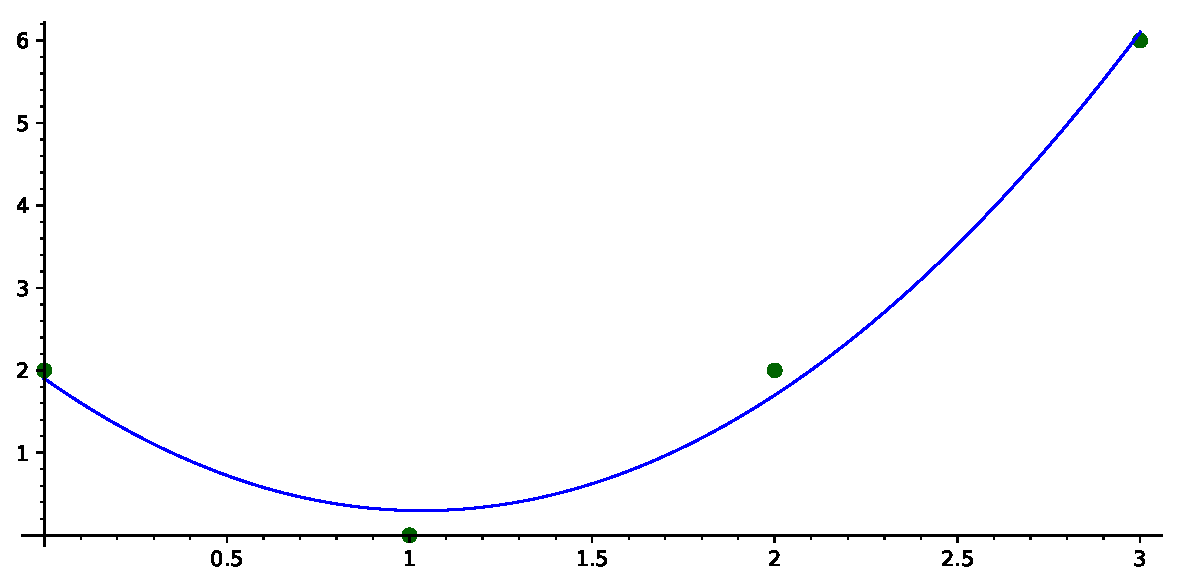
\includegraphics[width=5in]{leastsquares}
\]

\end{solution} 
\ee
